\chapter{狀態方程式、輻射與真空能}

\lectureoverview{均勻宇宙的演化，在很大程度上就是尺度因子 \(a(t)\) 的演化。弗里德曼方程提供幾何描述，而物質的狀態方程式則告訴我們，空間膨脹時能量密度如何變化。我們先從流體做功推導 \(\rho\propto a^{-3(1+w)}\)，再藉由計算光子動量的傳遞得到輻射的 \(P=\rho/3\)，最後由 \(P=-\rho\) 確認真空能。正的真空能會造成德西特膨脹；曲率與宇宙學常數的正負號則會帶來反彈與再坍縮解，並可將這些解視為簡單的力學系統。}

\section{尺度因子與缺少的物質定律}

先回顧一下我們接下來要做什麼。在均勻且各向同性的近似下，宇宙的主要演化歷程由一個函數 \(a(t)\) 描述。知道這個函數並不能回答所有關於宇宙的問題，但它決定了距離、膨脹速率，以及大尺度宇宙各個時期的演變順序。本講的目的還不是根據觀測確立這些時期，而是從基本物理出發，推導出使這些模型得以成立的狀態方程式。

我們已經看過兩個基準模型：
\begin{equation}
a(t)\propto t^{2/3}
\qquad\text{(matter domination)},
\end{equation}
以及
\begin{equation}
a(t)\propto t^{1/2}
\qquad\text{(radiation domination)}.
\end{equation}
這兩條定律並非在所有時期都精確成立。輻射提供了有用的早期近似，物質則提供了較晚中期的近似；真空能最終又會改變晚期的行為。眼前要問的不是觀測如何揭示這些時期，而是弗里德曼方程右側相應的各項有何不同。

\begin{figure}[htbp]
\centering
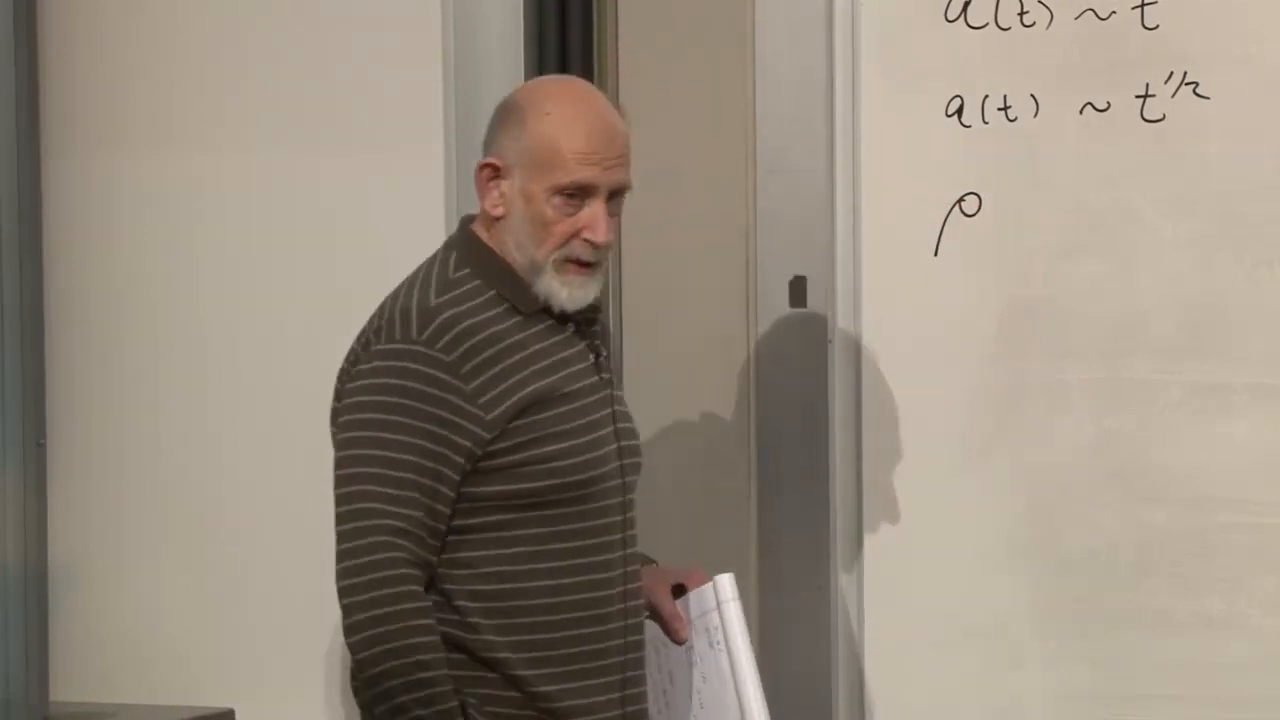
\includegraphics[width=0.72\textwidth]{lecture_05_figure_02.png}
\caption{回顧尺度因子的冪次定律，並引入新的密度符號。這是過渡階段的板書，推導尚未完成。}
\label{fig:c05-review-board}
\lectureframe{00:03:18.380}
\end{figure}

缺少的關鍵是狀態方程式。它決定弗里德曼方程右側的能量密度如何隨尺度因子變化。兩條基準定律是
\begin{equation}
\rho_{\text{matter}}=\frac{\rho_0}{a^3},
\qquad
\rho_{\text{rad}}=\frac{\rho_0}{a^4}.
\label{eq:c05-benchmark-densities}
\end{equation}
物質的密度會隨體積增大而稀釋，而體積與 \(a^3\) 成正比。輻射的密度則會再多減少一個 \(a\) 的冪次。我們要從壓力與能量密度的關係，理解這兩條定律如何導出。

\section{從壓力到密度標度定律}

一般而言，狀態方程式可能涉及密度、壓力、溫度及其他變數。對於此處討論的宇宙學成分，我們採用一種方便的常數 \(w\) 形式：
\begin{equation}
P=w\rho,
\label{eq:c05-eos}
\end{equation}
其中 \(w\) 用來描述流體的性質。板書使用大寫的 \(W\)；我們則採用慣用的小寫 \(w\)。這種線性形式涵蓋了下文的重要情形，但它只是簡化假設，並非所有可能的流體都遵守的定律。

對非相對論性物質而言，能量密度由靜止能量主導。若 \(n\) 是數密度，而 \(m\) 是粒子質量，則可概略寫成
\begin{equation}
\rho\simeq nmc^2.
\end{equation}
因子 \(c^2\) 使得即使很小的靜止質量也能成為龐大的能量來源；一粒塵埃若完全湮滅，釋放的能量也可達宏觀尺度。相較之下，壓力來自粒子撞擊壁面時傳遞的動量，其量級為 \(nmv^2\)。保齡球傳遞的動量比乒乓球大，但對冷氣體而言，所有相關速度都滿足 \(v\ll c\)。因此
\begin{equation}
\frac{P}{\rho}\sim\frac{v^2}{c^2}\ll1,
\qquad
w\simeq0.
\label{eq:c05-dust-eos}
\end{equation}
輻射以 \(c\) 運動，因此不適用這項近似。我們將推導它的 \(w\) 值，而不是直接假設。

現在需要一套通用方法，將方程~\eqref{eq:c05-eos}轉換為 \(\rho\) 的標度定律。一個實驗室用的盒子就足以說明。星系當然不能真的放進盒子裡，但經過粗粒化處理後，它們的行為就像粒子；能量與壓力的關係也可以在局部推導。

\begin{figure}[htbp]
\centering
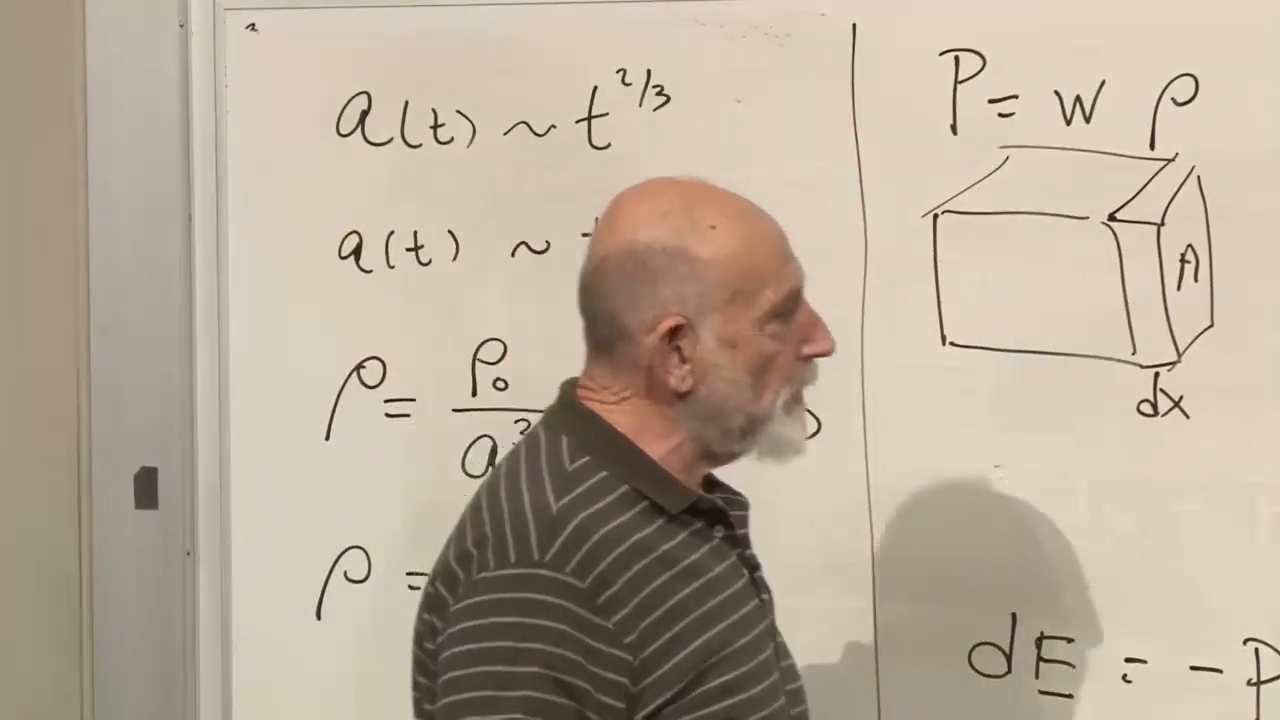
\includegraphics[width=0.86\textwidth]{lecture_05_figure_03.png}
\caption{板書同時呈現狀態方程式、回顧過的密度標度關係，以及熱力學盒子的示意。講師遮住了部分先前的板書，因此此圖用來呈現版面與可見方程式，而非完整轉錄。}
\label{fig:c05-box-board}
\lectureframe{00:13:39.612}
\end{figure}

板書左側是回顧過的宇宙學標度關係，右側則開始討論盒子。合起來看，可見內容連結了
\begin{equation}
\rho_{\text{matter}}=\frac{\rho_0}{a^3},
\qquad
\rho_{\text{rad}}=\frac{\rho_0}{a^4},
\qquad
P=w\rho.
\end{equation}
我們要從狀態方程式推導出這兩條密度定律。

其中一面牆的面積為 \(A\)。將牆向外移動 \(dx\)，於是
\begin{equation}
dV=A\,dx.
\end{equation}
壓力是單位面積所受的力，因此作用在牆上的力為 \(PA\)。氣體做功 \(PA\,dx=P\,dV\)，使盒內剩餘的能量減少。
\begin{equation}
dE=-P\,dV.
\label{eq:c05-work-law}
\end{equation}
\begin{figure}[htbp]
\centering
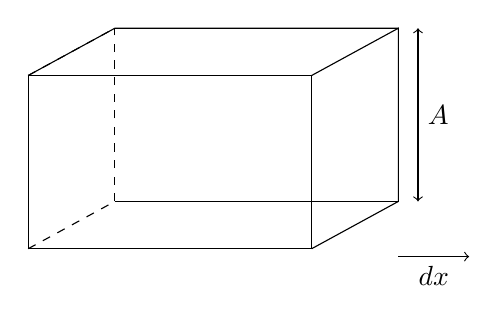
\begin{tikzpicture}[scale=1.0]
\draw (0,0) -- (3.6,0) -- (3.6,2.2) -- (0,2.2) -- cycle;
\draw (3.6,0) -- (4.7,0.6) -- (4.7,2.8) -- (3.6,2.2);
\draw (0,2.2) -- (1.1,2.8) -- (4.7,2.8);
\draw (1.1,0.6) -- (4.7,0.6);
\draw[dashed] (0,0) -- (1.1,0.6);
\draw[dashed] (0,2.2) -- (1.1,2.8);
\draw[dashed] (1.1,0.6) -- (1.1,2.8);
\draw[<->] (4.95,0.6) -- (4.95,2.8);
\node[right] at (4.95,1.7) {\(A\)};
\draw[->] (4.7,-0.1) -- (5.6,-0.1);
\node[below] at (5.15,-0.1) {\(dx\)};
\end{tikzpicture}
\caption{熱力學盒子的清晰重繪圖，標示了面積為 \(A\) 的壁面與位移 \(dx\)。}
\label{fig:c05-box-redraw}
\end{figure}

總能量為
\begin{equation}
E=\rho V.
\end{equation}
微分可得
\begin{equation}
d(\rho V)=\rho\,dV+V\,d\rho.
\end{equation}
代入方程~\eqref{eq:c05-work-law}，得到
\begin{equation}
\rho\,dV+V\,d\rho=-P\,dV.
\end{equation}
再代入 \(P=w\rho\)：
\begin{equation}
V\,d\rho=-(1+w)\rho\,dV.
\end{equation}
這是導向所需方程式的中間結果，但還差一步。兩邊除以 \(\rho V\)。
\begin{equation}
\frac{d\rho}{\rho}=-(1+w)\frac{dV}{V}.
\end{equation}
\begin{figure}[htbp]
\centering
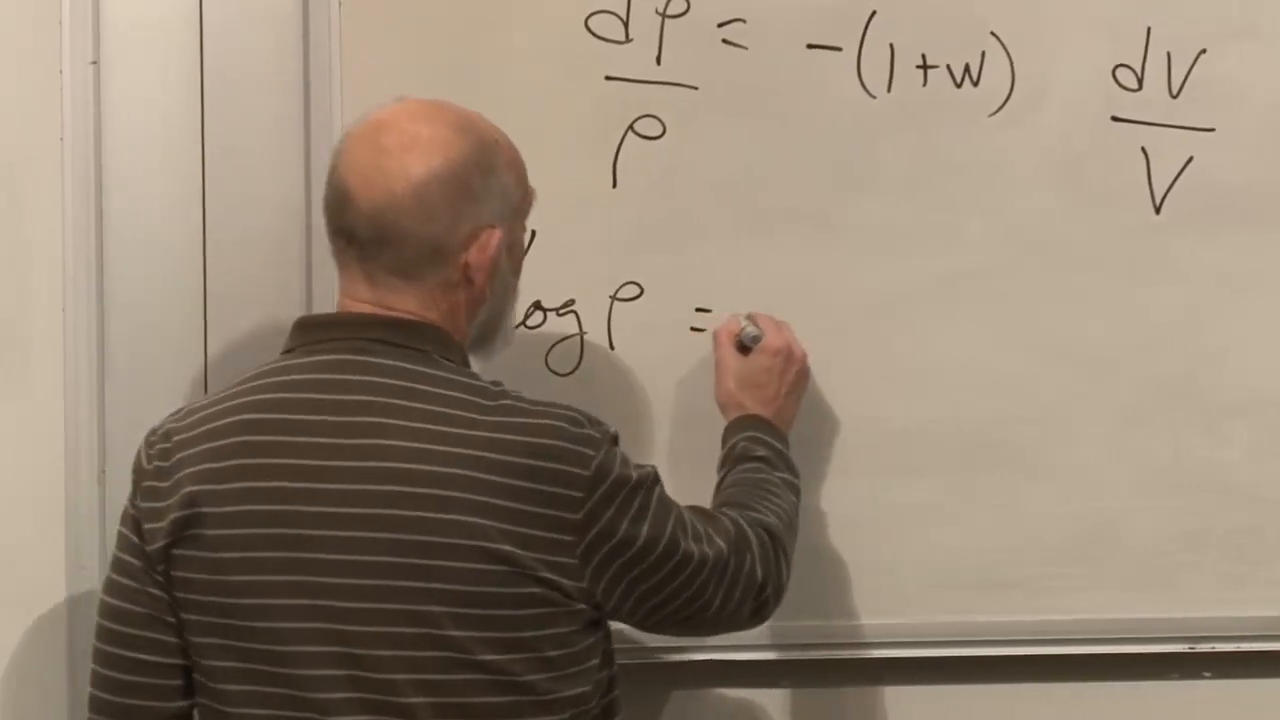
\includegraphics[width=0.78\textwidth]{lecture_05_figure_04.png}
\caption{將密度與體積分離後的方程式，以及對數積分的開頭。完整的右側是根據前述代數推導重建，並非取自被遮住的影像內容。}
\label{fig:c05-log-board}
\lectureframe{00:15:35.600}
\end{figure}

畫面顯示了分離變數後的方程式，以及 \(\log\rho=\) 的開頭。直接完成積分：
\begin{equation}
d(\log\rho)=-(1+w)\,d(\log V),
\end{equation}
於是
\begin{equation}
\log\rho=-(1+w)\log V+\text{const.}
\end{equation}
取指數後，得到
\begin{equation}
\rho\propto V^{-(1+w)}.
\end{equation}
這就是密度與體積的關係。

現在從盒子回到宇宙學。只移動一面牆是為了方便推導，並不代表我們假設宇宙具有各向異性。若三個方向均勻膨脹，得到的做功關係相同，而共動體積的變化為
\begin{equation}
V\propto a^3.
\end{equation}
因此
\begin{equation}
\boxed{\rho\propto a^{-3(1+w)}}.
\label{eq:c05-density-scaling}
\end{equation}
在 \(d\) 個空間維度中，指數 \(3\) 會改為 \(d\)；推導的其餘部分不變。

\section{初步應用：物質與輻射}

現在可以把先前回顧的公式作為推論導出，而不是將它們當成假設。

對非相對論性物質，取
\begin{equation}
w=0.
\end{equation}
於是
\begin{equation}
\rho\propto a^{-3},
\end{equation}
這正是物質稀釋定律。

對輻射，暫且取
\begin{equation}
w=\frac13.
\end{equation}
若這個取值正確，則
\begin{equation}
\rho\propto a^{-3(1+1/3)}=a^{-4}.
\end{equation}
因此，多出的反比冪次相當於 \(w=1/3\)。尚待解決的是如何從光子物理推導出這個值。

\section{為什麼輻射壓力是其能量密度的三分之一}

輻射可以描述為電磁波，也可以描述為無質量粒子。我們以光子為例，計算盒中光子氣體的壓力。圖中的盒子畫成二維，但氣體本身及其角度分布是三維的。光子以光速運動，並在暫設的盒壁上彈性反射。

暫時假設所有光子的能量都相同，為 \(\epsilon\)。稍後將不同能量的貢獻加總時，就不需要這項簡化了。令 \(\vec{\pi}\) 表示光子的動量向量；我們不使用通常表示動量的符號 \(p\)，因為 \(P\) 已用來表示壓力。無質量粒子滿足以下關係：
\begin{equation}
\epsilon=c\,\pi,
\end{equation}
其中 \(\pi=|\vec{\pi}|\)。在本講採用的單位制中，\(c=1\)，所以
\begin{equation}
\epsilon=\pi.
\end{equation}
若 \(\nu\) 是光子數密度，則能量密度為
\begin{equation}
\rho=\epsilon\,\nu.
\end{equation}
令 \(x\) 軸垂直於其中一面牆。在短時間間隔 \(\Delta t\) 內，運動方向與該法線夾角為 \(\theta\) 的光子，只有在起始位置落於厚度為
\begin{equation}
\Delta x=\Delta t\cos\theta.
\end{equation}
的薄層內，才會到達牆面。光子反射時，其動量的 \(x\) 分量會反向，因此傳遞給牆面的動量為
\begin{equation}
\Delta \pi_x=2\epsilon\cos\theta.
\end{equation}
力是單位時間內傳遞的動量，因此一次撞擊對力的貢獻為 \(\Delta \pi_x/\Delta t\)。薄層內有 \(\nu A\Delta x\) 個光子，但只有一半朝牆面運動，所以相關的光子數為 \(\tfrac12 \nu A\Delta x\)。將總力除以牆面積 \(A\)，得到
\begin{align}
P(\theta)
&=
\frac{1}{A}
\left(\frac{2\epsilon\cos\theta}{\Delta t}\right)
\left(\frac12 \nu A\Delta x\right) \\
&=
\epsilon\nu\cos\theta\frac{\Delta x}{\Delta t} \\
&=
\epsilon\nu\cos^2\theta \\
&=
\rho\cos^2\theta.
\end{align}
結果會隨角度而變，因為這裡只計算沿單一方向運動的光子所造成的貢獻。

\begin{figure}[htbp]
\centering
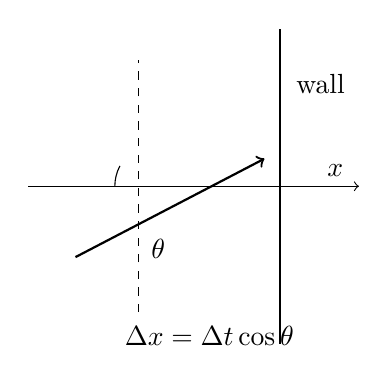
\begin{tikzpicture}[scale=1.0]
\draw[thick] (0,0) -- (0,4);
\draw[->] (-3.2,2) -- (1.0,2);
\node[above] at (0.7,2) {\(x\)};
\draw[dashed] (-1.8,0.4) -- (-1.8,3.6);
\node[below] at (-0.9,0.35) {\(\Delta x=\Delta t\cos\theta\)};
\draw[->,thick] (-2.6,1.1) -- (-0.2,2.35);
\node[below] at (-1.55,1.45) {\(\theta\)};
\draw (-2.1,2) arc[start angle=180,end angle=152,radius=0.55];
\node[right] at (0.08,3.3) {wall};
\end{tikzpicture}
\caption{光子以角度 \(\theta\) 入射到牆面時的動量，以及推導輻射壓力所用的幾何關係。}
\label{fig:c05-photon-pressure}
\end{figure}

對各向同性分布取平均。令 \(\mathbf n=(n_x,n_y,n_z)\) 為沿光子運動方向的單位向量。於是
\begin{equation}
n_x=\cos\theta,
\qquad
n_x^2+n_y^2+n_z^2=1.
\end{equation}
在各向同性氣體中，\(n_x^2\)、\(n_y^2\) 與 \(n_z^2\) 的平均值相等。對上述恆等式取平均，得到
\begin{equation}
\langle n_x^2\rangle+\langle n_y^2\rangle+\langle n_z^2\rangle=1,
\end{equation}
由對稱性，三項相等，因此
\begin{equation}
\langle n_x^2\rangle=\langle \cos^2\theta\rangle=\frac13.
\end{equation}
所以
\begin{equation}
P=\rho\langle \cos^2\theta\rangle=\frac{\rho}{3}.
\end{equation}
輻射的狀態方程式因此為
\begin{equation}
P=\frac13\rho,
\qquad
w=\frac13.
\end{equation}
因子 \(1/3\) 反映了平方後的單位向量分量由各個空間方向共同分攤。在 \(d\) 個各向同性空間維度中，同樣的推導會得到 \(\langle n_x^2\rangle=1/d\)。至此，完成了開頭所說的微觀推導。

\subsection{檢驗輻射推導的問題}

\begin{classroomqa}
\audiencequestion{所有光子的能量都必須相同嗎？}
\lecturerresponse{不必。對每個能量區間分別計算即可。每個區間的壓力都是其自身能量密度的三分之一，因此對整個光譜加總後，\(P=\rho/3\) 仍然成立。假設光子能量相同，只是為了簡化記號。\lecturetimestamp{00:39:08--00:39:36}}
\end{classroomqa}

\begin{classroomqa}
\audiencequestion{吸收輻射的黑色壁面，會得到與完美鏡面相同的結果嗎？空無一物的空間裡，壁面又是什麼？}
\lecturerresponse{處於熱平衡的黑色壁面會吸收並重新放出輻射，產生相同的平均動量平衡。宇宙空間並沒有實際的牆壁；這個表面只是想像中的邊界。每個向外穿出的光子，都有各向同性所提供的平均向內通量與之平衡，因此局部動量流的計算不變。課堂上討論的輻射主要是熱宇宙微波背景輻射，對這種輻射而言，熱平衡的圖像尤其自然。\lecturetimestamp{00:39:37--00:41:19}}
\end{classroomqa}

\begin{classroomqa}
\audiencequestion{量子統計會改變 \(P=\rho/3\) 嗎？}
\lecturerresponse{不會。玻色統計決定光子如何佔據可用的模態，因而決定光譜與總 \(\rho\)；但無質量粒子的各向同性應力仍為其能量密度的三分之一。\lecturetimestamp{00:41:51--00:42:02}}
\end{classroomqa}

\begin{classroomqa}
\audiencequestion{如果光子彼此散射，會怎樣？}
\lecturerresponse{一般的光子—光子散射極弱，因此在此處造成的修正可以忽略。在溫度與密度足夠高時，碰撞可能產生電子—正電子對，改變有效粒子種類與狀態方程式。這確實是一種效應，但它發生在遠比本論證所採用情況更高溫的環境。\lecturetimestamp{00:42:02--00:43:08}}
\end{classroomqa}

\begin{classroomqa}
\audiencequestion{壁面的面積 \(A\) 到哪裡去了？}
\lecturerresponse{中間步驟是單一光子造成的力乘上撞擊牆面的光子數，而光子數與 \(A\) 成正比。壓力等於力除以面積，因此最後除以 \(A\) 時，面積便約掉了。板書的疏漏在於太早把中間的算式稱為壓力；補上從力換算為壓力的步驟，就能修正這個問題。\lecturetimestamp{00:43:11--00:44:01}}
\end{classroomqa}

\section{負壓力與張力的意義}

到目前為止，粒子撞擊壁面並將壁面向外推。這種圖像自然會產生正壓力，但可能的情況並不僅止於此。

\begin{classroomqa}
\audiencequestion{能量密度本身可能為負嗎？}
\lecturerresponse{量子理論允許在特定限制條件下出現負能量密度，而宇宙學常數在形式上也可以取正值或負值。這些情況需要謹慎處理，並非我們此刻的起點。較熟悉的切入點是負\emph{壓力}：即使能量密度為正，壓力仍可能為負。\lecturetimestamp{00:44:25--00:44:59}}
\end{classroomqa}

\begin{classroomqa}
\audiencequestion{壓力怎麼可能是負的？}
\lecturerresponse{在一維世界中，盒子就是一段線段。自由運動的粒子在兩端反彈並向外推，形成正壓力。若改用拉緊的弦或彈簧連接兩端，將兩端拉開時，彈簧會把它們向內拉。這種向內的力就是張力，是負壓力的一維模型。\lecturetimestamp{00:45:04--00:46:31}}
\end{classroomqa}

\begin{figure}[htbp]
\centering
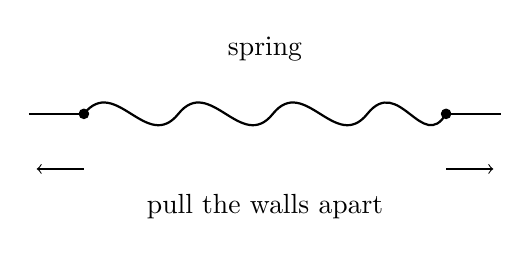
\begin{tikzpicture}[scale=1.0]
\draw[thick] (-3,0) -- (-2.3,0);
\draw[thick] (2.3,0) -- (3,0);
\draw[fill] (-2.3,0) circle (0.06);
\draw[fill] (2.3,0) circle (0.06);
\draw[thick] (-2.3,0)
.. controls (-1.9,0.5) and (-1.5,-0.5) .. (-1.1,0)
.. controls (-0.7,0.5) and (-0.3,-0.5) .. (0.1,0)
.. controls (0.5,0.5) and (0.9,-0.5) .. (1.3,0)
.. controls (1.7,0.5) and (2.0,-0.5) .. (2.3,0);
\draw[->] (-2.3,-0.7) -- (-2.9,-0.7);
\draw[->] (2.3,-0.7) -- (2.9,-0.7);
\node[below] at (0,-0.9) {pull the walls apart};
\node[above] at (0,0.55) {spring};
\end{tikzpicture}
\caption{以一維彈簧類比負壓力。}
\label{fig:c05-tension}
\end{figure}

功的計算也會相應反轉。膨脹時，正壓力氣體對外做功，內能因而減少。若向外拉動兩端以對抗張力，能量則會儲存在彈簧中。更一般地說，彼此吸引的成分可以相互牽引，並將邊界向內拉。因此，系統可以同時具有 \(\rho>0\) 和 \(P<0\)，因而得到 \(w<0\)，這並不矛盾。這種可能性至關重要，因為真空能恰好具有這樣的正負號組合。

\section{真空能與宇宙學常數}

真空能是歸屬於空間本身的能量。量子場論以場模態所對應諧振子的零點運動，為真空能提供了理論動機；不過，要描述其宏觀性質，並不需要先解決這個微觀問題。它的定義性質是：無論選擇哪個位置、哪種大小的區域，空無一物的空間都具有相同的能量密度。
\begin{equation}
\rho=\rho_0=\text{const.}
\label{eq:c05-vacuum-density}
\end{equation}
若一個體積為 \(V\) 的區域只含有真空能，則該區域的總能量為
\begin{equation}
E=\rho_0 V.
\end{equation}
\begin{classroomqa}
\audiencequestion{盒子限制了可允許的場模態，會因此改變真空密度嗎？}
\lecturerresponse{有限區域的總能量小於整個空間的總能量，因為該區域的體積較小；但體積能量密度 \(\rho_0\) 保持不變。真實邊界可能改變模態能量並產生卡西米爾效應，但只有在間距與相關波長相近時，這項修正才會顯著。它不是宇宙學所採用的大尺度真空密度。\lecturetimestamp{00:50:06--00:51:25}}
\end{classroomqa}

定義
\begin{equation}
\Lambda=\frac{8\pi G}{3}\rho_0.
\label{eq:c05-lambda-definition}
\end{equation}
這項定義將弗里德曼方程中出現的組合納入其中。反過來可得
\begin{equation}
\rho_0=\frac{3\Lambda}{8\pi G}.
\end{equation}
參數 \(\Lambda\) 就是宇宙學常數。驅動晚期加速、且近乎固定不變的成分，通常稱為暗能量。

尺度因子的依賴關係已經確定，因此現在反過來運用盒子論證，推知真空能的壓力。由於 \(d\rho_0=0\)，
\begin{equation}
dE=d(\rho_0V)=\rho_0\,dV.
\end{equation}
另一方面，熱力學的做功關係仍為
\begin{equation}
dE=-P\,dV.
\end{equation}
若令 \(P=w\rho_0\)，則
\begin{equation}
dE=-w\rho_0\,dV.
\end{equation}
比較兩式可得
\begin{equation}
w=-1.
\end{equation}
因此
\begin{equation}
P=-\rho.
\end{equation}
彈簧的類比正是在為這個正負號做準備。正真空能具有負壓力；負真空能則具有正壓力。天文觀測 \(w\)，是在檢驗晚期成分是否真的像不會稀釋的真空一樣：\(w\) 越接近 \(-1\)，其行為就越接近方程~\eqref{eq:c05-vacuum-density}。

\begin{classroomqa}
\audiencequestion{\(P=-\rho\)是空間為空時的狀態方程式嗎？我們能計算 \(\rho_0\) 嗎？}
\lecturerresponse{當真空能存在時，這就是空無一物的空間所遵循的狀態方程式。要計算其大小則困難得多。每一種量子場及每一個能量尺度都可能有所貢獻，包括尚未發現的場，因此目前沒有公認的計算能解釋觀測值。主要的謎題不是如何寫出 \(w=-1\)，而是為什麼淨 \(\rho_0\) 小得如此驚人。\lecturetimestamp{00:57:27--00:58:29}}
\end{classroomqa}

\section{弗里德曼動力學中的真空能}

如同先前分別考察純物質與純輻射，現在單獨考察真空能。令 \(\rho=\rho_0\)，弗里德曼方程便成為
\begin{equation}
\left(\frac{\dot a}{a}\right)^2=\Lambda-\frac{k}{a^2},
\label{eq:c05-vacuum-friedmann}
\end{equation}
其中 \(k=+1,0,-1\) 分別對應球面、平坦與雙曲空間。\(\Lambda\) 可正可負，再配合 \(k\) 的三種取值，總共有六種正負號組合；不過，並非每種組合都存在實數解。

\begin{remark}
本講採用的定義是 \(\Lambda=(8\pi G/3)\rho_0\)，因此此處 \(\Lambda\) 的量綱為 \(H^2\)。若採用常見的慣例 \(G_{\mu\nu}+\Lambda_{\mathrm E}g_{\mu\nu}=8\pi G T_{\mu\nu}\)，相應的參數則為 \(\Lambda_{\mathrm E}=3\Lambda\)。
\end{remark}

\subsection{平坦切片中的德西特膨脹}

令 \(k=0\)。於是
\begin{equation}
\left(\frac{\dot a}{a}\right)^2=\Lambda.
\end{equation}
當 \(\Lambda>0\) 時，選擇膨脹分支：
\begin{equation}
\dot a=\sqrt{\Lambda}\,a,
\end{equation}
因此
\begin{equation}
a(t)=C\,e^{\sqrt{\Lambda}\,t}.
\end{equation}
此時哈勃參數為常數：
\begin{equation}
H=\frac{\dot a}{a}=\sqrt{\Lambda}.
\end{equation}
這是平坦切片中的德西特空間。它以 Willem de Sitter 命名；愛因斯坦於 1917 年引入宇宙學常數後不久，de Sitter 就找到了這個解。若 \(\Lambda<0\) 且 \(k=0\)，方程~\eqref{eq:c05-vacuum-friedmann}沒有實數解，因為 \(H^2\) 不可能為負。

\begin{classroomqa}
\audiencequestion{這裡的哈勃參數真的為常數嗎？這個時空有大爆炸嗎？}
\lecturerresponse{對純粹的平坦切片解而言，\(H=\sqrt{\Lambda}\) 確實是常數。雖然只有在 \(t\to-\infty\) 時 \(a(t)\to0\)，但這個座標區域並非測地完備：某些朝過去方向延伸的軌跡，會在有限的固有時間內抵達其邊界。因此，單靠這個公式無法判定整體時空是否有大爆炸。完整的德西特幾何不只包含這個平坦切片；這一點要等到詳細研究幾何時再討論。\lecturetimestamp{01:06:54--01:08:07}}
\end{classroomqa}

包含物質、輻射、曲率與真空能的宇宙，其弗里德曼方程可概略寫成
\begin{equation}
\left(\frac{\dot a}{a}\right)^2
=
\Lambda+\frac{C_m}{a^3}+\frac{C_r}{a^4}-\frac{k}{a^2}.
\label{eq:c05-mixed-friedmann}
\end{equation}
在早期，當 \(a\) 很小時，反比冪次項占主導，真空能可以忽略。到了晚期，當 \(a\) 很大時，常數項 \(\Lambda\) 占主導。因此宇宙會經歷轉變：早期由物質或輻射主導，晚期則趨近德西特式的行為。

指數函數滿足 \(\ddot a>0\)，因此真空能主導時，膨脹會加速。在過渡期間，加速度不必恰好呈指數形式，因為物質仍會對方程~\eqref{eq:c05-mixed-friedmann}有所貢獻。講座當時的觀測顯示，宇宙正處於這些成分相互競爭的階段，尚未進入純粹的德西特時期。

\section{關於真空能的問題}

\begin{classroomqa}
\audiencequestion{如果真空能是基態能量，怎麼可能為負？}
\lecturerresponse{玻色振子模態的貢獻為 \(+\tfrac12\hbar\omega\)，而費米子模態的貢獻符號相反。淨真空能是許多場與能量尺度的貢獻總和，因此在總和確定之前，正負兩種結果都有可能。這些貢獻的存在並不意外；困難的是解釋為什麼最後剩下的值小得如此驚人。\lecturetimestamp{01:12:00--01:14:12}}
\end{classroomqa}

\begin{classroomqa}
\audiencequestion{若 \(w=-1\) 為常數，未來會發生大撕裂嗎？}
\lecturerresponse{不會。若宇宙學常數滿足 \(w=-1\)，宇宙會呈現德西特式的指數膨脹，但不會出現稱為大撕裂的有限時間發散。大撕裂屬於一種假想的幽靈成分，其 \(w<-1\)，因此密度會隨宇宙膨脹而增加。此處並未假設有這種成分。\lecturetimestamp{01:14:13--01:15:50}}
\end{classroomqa}

\begin{classroomqa}
\audiencequestion{精確的超對稱能讓真空能消失嗎？}
\lecturerresponse{可以，因為每個玻色自由度都會與一個費米自由度配對，從而抵銷零點能貢獻。然而，自然界並未呈現精確的低能超對稱：觀測到的玻色子與費米子並非質量相同的超對稱夥伴。因此，精確抵銷無法解釋目前觀測到的世界中的真空能。\lecturetimestamp{01:15:51--01:16:20}}
\end{classroomqa}

\begin{classroomqa}
\audiencequestion{自然估算的真空能與觀測值之間，差距有多大？}
\lecturerresponse{普適常數 \(c\)、\(\hbar\) 與 \(G\) 定義了普朗克單位。光速 \(c\) 限制所有訊號的傳播速度，\(\hbar\) 決定普適的量子不確定性尺度，而 \(G\) 將所有能量與重力耦合。利用這些常數，可以構造出量級約為 \(10^{-5}\) 克的普朗克質量，以及量級約為 \(10^{-33}\) 公分的普朗克長度；據此得到的普朗克能量密度，約等於每立方普朗克長度含有一個普朗克能量。講座中以這些單位表示的觀測真空密度約為 \(10^{-123}\)，確切指數則視採用的慣例而定。謎題在於，為什麼自然尺度所暗示的巨大貢獻，最後只留下如此微小但不為零的結果。\lecturetimestamp{01:16:21--01:23:12}}
\end{classroomqa}

\begin{classroomqa}
\audiencequestion{既然預期真空會有能量貢獻，物理學家為何會對非零宇宙學常數的發現感到驚訝？}
\lecturerresponse{觀測結果經過一次又一次改進，卻始終與零相符。這段歷史使人們在心理上預期，某個尚未知曉的精確原理——或許出自未來的量子重力理論——會強制使所有貢獻完全抵銷。後來的探測結果推翻了這項預期。這種驚訝反映的是數十年來愈發嚴格、始終與零相符的觀測結果，而不是由某種推導得出真空能必須為零。\lecturetimestamp{01:23:14--01:26:05}}
\end{classroomqa}

\begin{classroomqa}
\audiencequestion{觀測能否判定暗能量是否隨時間改變？}
\lecturerresponse{觀測無法排除遙遠未來發生突變，但可以比較過去數十億年間的膨脹歷史。測量 \(w\)，或更一般地測量 \(w(a)\)，可以檢驗密度在這段期間是否演化。講座報告的當時限制約為百分之十；這是歷史數值，而持續適用的重點是，\(w=-1\) 對應於密度不隨時間改變。\lecturetimestamp{01:26:06--01:27:16}}
\end{classroomqa}

\begin{classroomqa}
\audiencequestion{若空間維度數不同，結果會有何差異？}
\lecturerresponse{整體結構仍然相同。在 \(d\) 個各向同性空間維度中，輻射滿足 \(w=1/d\)，密度隨 \(a^{-(d+1)}\) 稀釋，而符合洛倫茲不變性的真空能仍滿足 \(w=-1\)。弗里德曼方程中的數值係數會隨維度改變，但稀釋中的物質、輻射與不稀釋的真空之間的區別仍然成立。\lecturetimestamp{01:27:16--01:27:57}}
\end{classroomqa}

\section{曲率與力學類比}

\subsection{正曲率與正真空能}

取 \(k=+1\) 與 \(\Lambda>0\)：
\begin{equation}
\left(\frac{\dot a}{a}\right)^2=\Lambda-\frac{1}{a^2}.
\label{eq:c05-closed-vacuum}
\end{equation}
兩邊乘以 \(a^2\)，得到
\begin{equation}
\dot a^2-\Lambda a^2=-1.
\label{eq:c05-inverted-oscillator}
\end{equation}
把 \(a\) 視為一個假想粒子的座標。此時 \(\dot a^2\) 是它的動能項，\(-\Lambda a^2\) 是向下開口的二次位能，而總能量為 \(-1\)。物理上允許的分支滿足 \(a\geq\Lambda^{-1/2}\)：宇宙從大尺度開始收縮，在最小尺度處暫停，隨後再次膨脹。

精確解為
\begin{equation}
a(t)=\Lambda^{-1/2}\cosh(\sqrt{\Lambda}\,t).
\label{eq:c05-closed-desitter}
\end{equation}
利用
\begin{equation}
\cosh(\sqrt{\Lambda}\,t)
=
\frac12\left(e^{\sqrt{\Lambda}\,t}+e^{-\sqrt{\Lambda}\,t}\right),
\end{equation}
這個函數對時間呈對稱。在 \(t=0\) 時，\(a=\Lambda^{-1/2}\)；沿時間的任一方向前進，尺度因子都會指數增長。因此，閉合切片呈現出收縮、非奇異的最小尺度，以及再膨脹。它在整體上看起來與平坦指數膨脹切片不同，但兩種座標系描述的是同一德西特幾何的不同部分。

\subsection{負宇宙學常數}

令 \(\Lambda=-|\Lambda|\)。若 \(k=+1\)，則方程~\eqref{eq:c05-vacuum-friedmann}的右側對所有 \(a\) 都是負值，但 \(H^2\geq0\)。因此，這種純真空類型不存在實數的 FRW 解。

當 \(k=-1\) 時，
\begin{equation}
\left(\frac{\dot a}{a}\right)^2=-|\Lambda|+\frac{1}{a^2}.
\end{equation}
兩邊乘以 \(a^2\)，得到
\begin{equation}
\dot a^2+|\Lambda|a^2=1.
\label{eq:c05-negative-lambda-oscillator}
\end{equation}
這就是簡諧振子的能量方程。由於 \(a\geq0\)，物理上可行的半個週期為
\begin{equation}
a(t)=\frac{1}{\sqrt{|\Lambda|}}
\sin\!\left(\sqrt{|\Lambda|}\,t\right),
\qquad
0<t<\frac{\pi}{\sqrt{|\Lambda|}}.
\end{equation}
開放宇宙從 \(a=0\) 開始，膨脹至 \(a_{\max}=|\Lambda|^{-1/2}\)，接著回到大坍縮。因此，開放的空間幾何並不保證宇宙永遠膨脹；負宇宙學常數可以使膨脹反轉。非常大的正 \(\Lambda\) 會撕裂束縛結構，而很大的負值則會造成快速再坍縮。

\begin{figure}[htbp]
\centering
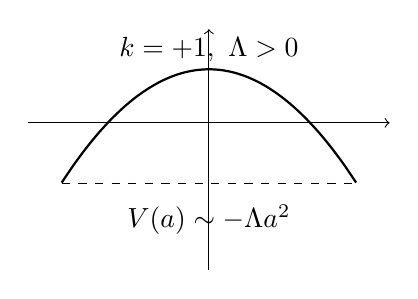
\begin{tikzpicture}[scale=0.85]
\draw[->] (-2.7,0) -- (2.7,0);
\draw[->] (0,-2.2) -- (0,1.4);
\draw[thick,domain=-2.2:2.2,smooth] plot (\x,{-0.35*(\x)^2 + 0.8});
\draw[dashed] (-2.2,-0.9) -- (2.2,-0.9);
\node at (0,-1.45) {\(V(a)\sim -\Lambda a^2\)};
\node at (0,1.1) {\(k=+1,\ \Lambda>0\)};
\end{tikzpicture}
\hspace{2em}
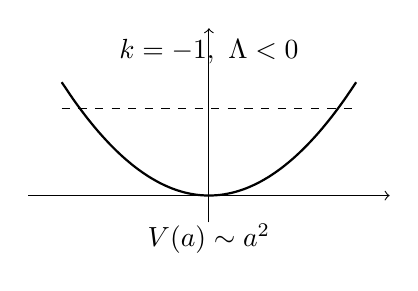
\begin{tikzpicture}[scale=0.85]
\draw[->] (-2.7,0) -- (2.7,0);
\draw[->] (0,-0.4) -- (0,2.5);
\draw[thick,domain=-2.2:2.2,smooth] plot (\x,{0.35*(\x)^2});
\draw[dashed] (-2.2,1.3) -- (2.2,1.3);
\node at (0,-0.65) {\(V(a)\sim a^2\)};
\node at (0,2.15) {\(k=-1,\ \Lambda<0\)};
\end{tikzpicture}
\caption{閉合德西特反彈與開放宇宙在負 \(\Lambda\) 下再坍縮的示意有效位能。}
\label{fig:c05-mechanical-potentials}
\end{figure}

\begin{classroomqa}
\audiencequestion{這些 Friedmann 方程真的是 Einstein 方程嗎？}
\lecturerresponse{是的。均勻性與各向同性將度規簡化為單一函數\(a(t)\)後，所得方程就是 Einstein 場方程。對稱性約化消去了大部分張量分量，只留下這個描述宇宙膨脹的常微分方程。\lecturetimestamp{01:43:52--01:44:05}}
\end{classroomqa}

\begin{classroomqa}
\audiencequestion{尺度因子\(a\)可能是複數嗎？}
\lecturerresponse{在此處探討的實數值經典 FRW 宇宙學中，不可能。尺度因子表示空間大小，因此取為實數且非負。複化幾何可能出現在其他數學方法中，但與本講所討論的解無關。\lecturetimestamp{01:44:06--01:44:21}}
\end{classroomqa}

\begin{classroomqa}
\audiencequestion{壓力必須是密度的線性函數，有什麼物理上的理由嗎？}
\lecturerresponse{沒有。令\(w\)為常數很方便，而且恰好適用於此處考慮的主要成分。物質、輻射與真空組成的混合物，其\(w\)不會在所有宇宙時期都維持同一常數；一般物質的\(P(\rho)\)也可能是非線性的。對於正壓流體，在\(c=1\)的單位制下，\(dP/d\rho\)決定聲速平方；若\(w\)為常數，這個導數便是常數，但自然界不必遵循這種情形。\lecturetimestamp{01:44:21--01:45:34}}
\end{classroomqa}

\section{本節要點}

狀態方程將微觀物理與尺度因子的時間演化聯繫起來。共動盒中的絕熱作功給出
\[
\rho\propto a^{-3(1+w)}.
\]
冷物質滿足\(w=0\)，且\(\rho\propto a^{-3}\)。各向同性的光子動量通量給出
\[
\left\langle\cos^2\theta\right\rangle=\frac13,
\qquad
P_{\mathrm r}=\frac{\rho_{\mathrm r}}{3},
\qquad
\rho_{\mathrm r}\propto a^{-4}.
\]

張力讓負壓力在物理上變得容易理解。恆定的真空密度滿足
\[
P_\Lambda=-\rho_\Lambda,
\qquad
w_\Lambda=-1.
\]
正真空能量在平坦切片中造成指數型的 de Sitter 膨脹，在閉合切片中則造成\(\cosh\)型反彈。負真空能量甚至能使開放宇宙重新坍縮。無論真空能量的符號為何，Friedmann 方程都可視為有效的力學能量方程。尚未解決的問題不是量子場為何會貢獻真空能量，而是為何觀測到的淨貢獻幾乎為零，卻又不恰好為零。
